\chapter{基于集中平台的iBGP系统结构}
\label{cha:china}


\section{本章引言}
可扩展问题是互联网iBGP协议的重要问题,随着网络规模和需求的不断增加,大多数自治系统已经不采用传统的Full-mesh的iBGP连接结构,而是使用配置比较方便、技术比较成熟的路由反射。现有的解决iBGP可扩展问题的思路可分为两种:分布式路由体系结构、集中式路由体系结构。分布式路由体系结构下的相关研究主要有路由反射和AS联邦,其解决了iBGP的可扩展问题,但是带来了新的问题,比如:非最优出口、转发环路、路由震荡。而集中式路由体系结构的相关研究主要有SoftRouter、RCP、RFCP三种代表性方案,这三种方案解决了iBGP的可扩展问题,但也分别存在集中平台本身的可扩展性差、路由存储冗余重复、未优化的传统路由计算方式等等问题。

本文基于数据平面和控制平面分离的思想,提出了基于集中平台的iBGP系统结构,将自治系统内部的路由存储、策略管理、路由计算以及路由转发交换功能合理划分为集中平台和自治系统内边界路由器上执行的两部分。该基于集中平台的iBGP系统结构处理路由信息的基本流程为:
\begin{itemize}
  \item 自治系统内的边界路由器收到路由信息,通过iBGP协议将从eBGP经过收到的路由信息发送到集中平台;
  \item 集中平台执行路由信息存入路由信息表Adj-RIB-In、将路由信息进行入站过滤后存入Loc-RIB、为每台自治系统内的边界路由器计算出最优路由、进行出站过滤等操作;
  \item 集中平台上将过滤后的最优路由传输给域内的每台边界路由器,边界路由器将收到的路由信息通过eBGP连接宣告出去。
\end{itemize}

集中式路由体系结构下,路由存储、策略管理、路由计算等存在很多优化空间。本文提出的基于集中平台的iBGP系统,不仅解决了iBGP存在的可扩展问题,而且对自治系统内BGP的路由存储和路由计算进行了优化。

本章首先提出基于集中平台的iBGP系统架构,之后对系统中的两个主要模块增量路由存储、复式路由计算进行详细的介绍,最后主要从解决iBGP可扩展问题、与分布式路由体系结构方案的对比、与集中式路由体系结构方案的这三个方面对基于集中平台的iBGP系统进行定性的分析。



\begin{figure}
  \centering
  % Requires \usepackage{graphicx}
  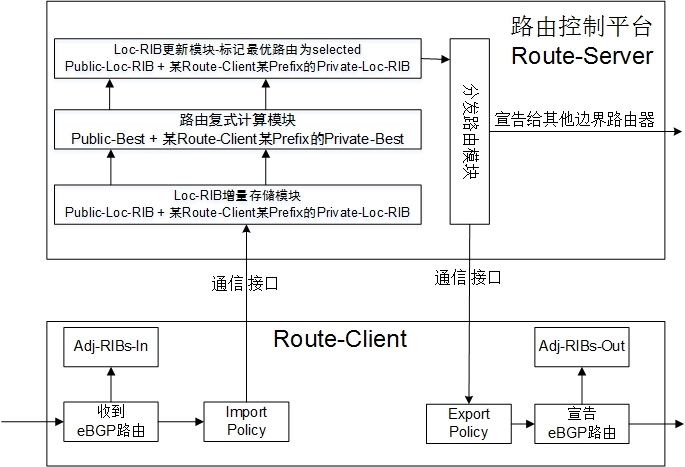
\includegraphics[width=\textwidth]{rscp-ibgp}
  \caption{RSCP-iBGP系统架构图}
  \label{fig:rscp-ibgp}
\end{figure}

\section{新型iBGP路由系统}
本文提出的自治系统内部的基于集中平台的iBGP新架构命名为RSCP-iBGP(Route Server Control Platform iBGP)。RSCP-iBGP基本思想是将自治系统内边界路由器的控制平面和数据平面分离,将边界网关协议BGP中的路由计算、路由存储、路由策略从边界路由器中剥离出来,交由独立的、且逻辑比较集中的运行在路由控制平台的Route-Server执行,而自治系统内部的普通边界路由器作为Route-Client对路由信息进行接收转发等操作。RSCP-iBGP系统如图\ref{fig:rscp-ibgp},这个系统运行在自治系统内部,主要包含三部分:自治系统内部的路由控制平台(Route-Server),自治系统内部的多台边界路由器(Route-Client),以及自治系统内部边界路由器与路由控制平台的标准通信接口(iBGP协议):
\begin{itemize}
  \item 通信协议使用iBGP协议,来传输BGP路由信息;
  \item 路由控制平台上运行1台Route-Server进行集中式的路由存储、策略管理、路由计算。当Route-Server收集路由模块,收集到自治系统内部边界路由器Route-Client-Ri发来的更新路由消息,Route-Server现将该路由加入Adj-RIB-In表,之后该路由经过Route-Client-Ri的入站策略后进入Loc-RIB增量存储模块,存储经过入站策略的路由信息,将Loc-RIB表以及IGPcost值输入路由复式计算模块,得到自治系统每台边界路由的针对该前缀的最优路由,之后在路由集中控制平台上分别经过每台边界路由器的出站策略,将其结果输入到分发路由模块,分发路由模块则分别将经过出站策略的该前缀的最优路由传输给自治系统内的每台边界路由;
  \item 自治系统内部的边界路由器Route-Cleint:当收到eBGP路由时,将其通过iBGP协议发送给路由控制平台上的Route-Server;当收到路由控制平台上的Route-Server发来的iBGP路由时,Route-Client将其宣告给自己的所有eBGP邻居。
\end{itemize}

\section{系统模块介绍}
\subsection{路由增量存储模块}
\subsection{路由复式计算模块}
\section{理论分析}
\subsection{解决iBGP可扩展问题}
假设某自治系统有N台边界路由器,在传统Full-mesh的iBGP结构中,域内自治系统需要建立N(N-1)/2数量的BGP连接。该自治系统的拓扑结构对应到本文的RSCP-iBGP系统结构,自制系统内的有N台Route-client边界路由器用于接受转发其他自治系统传输过来的路由、1台或者多台运行在路由控制平台的Route-Server用于路由存储和路由计算等操作,N台Route-Client与1台Route-Server建立N个扩展的iBGP连接来传输BGP路由信息,则该基于集中平台的iBGP新架构解决了iBGP协议可扩展性差的问题。


\subsection{与分布式路由体系结构方案的对比}
\subsection{与集中式路由体系结构方案的对比}
\subsection{总结}

\section{本章小结}
总结